\documentclass[../main/main.tex]{subfiles}

\begin{document}
\bab{STUDI LITERATUR}

\subsection{Kamus Dwibahasa}
\label{subbab:studi_kamus}
Istilah "kamus dwibahasa" digunakan sebagai padanan istilah bahasa Inggris "\textit{bilingual dictionary}". Menurut kamus Oxford \textit{online}\footnote{\url{http://www.oxforddictionaries.com}}, definisi kata "\textit{bilingual}" adalah teks atau aktivitas yang dituliskan atau dilakukan dalam dua bahasa, sedangkan kata "\textit{dictionary}" didefinisikan sebagai sebuah buku atau sumber elektronik yang mendaftarkan kata-kata dari sebuah bahasa (biasanya terurut sesuai abjad) dan memberikan padanan katanya dalam bahasa yang lain.

Menurut KBBI (Kamus Besar Bahasa Indonesia) \textit{online}\footnote{\url{http://kbbi.web.id/}}, definisi dari istilah "kamus dwibahasa" adalah kamus yang memuat kata atau gabungan kata suatu bahasa yang disusun secara alfabetis dengan penjelasan makna dan contoh pemakaiannya di dalam bahasa lain yang menjadi bahasa sasaran. Dari ketiga definisi tersebut, dapat ditarik kesimpulan bahwa setidaknya terdapat 5 unsur utama yang ada di dalam sebuah kamus dwibahasa, yaitu
\begin{enumerate}
\item bahasa asal,
\item bahasa sasaran,
\item daftar kata atau frasa bahasa asal,
\item daftar kata atau frasa bahasa sasaran, dan
\item translasi antara kata atau frasa bahasa asal dengan bahasa sasaran.
\end{enumerate}

Selain itu, \textcite{limanthie} dalam tugas akhirnya menyebutkan, "Terdapat dua jenis kamus \textit{bilingual}, yaitu kamus \textit{unidirectional} dan kamus \textit{bidirectional}. Kamus \textit{unidirectional} hanya berisi terjemahan dari satu bahasa ke bahasa lain. Sedangkan kamus \textit{bidirectional} berisi terjemahan dari satu bahasa ke bahasa lain dan sebaliknya." Contoh entri kamus dwibahasa diberikan pada Tabel \ref{tbl:studi_kamus}. Contoh kamus tersebut masuk ke dalam jenis \textit{unidirectional} karena hanya menyediakan translasi dari bahasa Indonesia ke bahasa Jepang.

\begin{table}[htbp]
	\centering
	\caption{Contoh entri kamus dwibahasa}
	\label{tbl:studi_kamus}
	\begin{tabular}{|r|l|l|l|}
		\hline
		\textbf{No.} & \textbf{Bahasa Indonesia} & \textbf{Bahasa Jepang} & \textbf{Transliterasi}\\ \hline
		\tableitem. & bahasa pemrograman & \begin{CJK}{UTF8}{min}プログラミング言語\end{CJK} & puroguramingu gengo\\ \hline
		\tableitem. & kamera digital & \begin{CJK}{UTF8}{min}デジカメ\end{CJK} & dejikame\\ \hline
		\tableitem. & kendaraan & \begin{CJK}{UTF8}{min}車\end{CJK} & kuruma\\ \hline
		\tableitem. & komputer & \begin{CJK}{UTF8}{min}コンピューター\end{CJK} & konpyu-ta-\\ \hline
		\tableitem. & mobil & \begin{CJK}{UTF8}{min}車\end{CJK} & kuruma\\ \hline
		\tableitem. & motor & \begin{CJK}{UTF8}{min}オートバイ\end{CJK} & o-tobai\\ \hline
		\tableitem. & motor & \begin{CJK}{UTF8}{min}単車\end{CJK} & tansha\\ \hline
		\tableitem. & motor & \begin{CJK}{UTF8}{min}モーター\end{CJK} & mo-ta-\\ \hline
	\end{tabular}
\end{table}

\subsection{Korpus}
Korpus (atau korpora dalam bentuk jamak) dapat didefinisikan sebagai sekumpulan sumber teks atau suara yang dapat dibaca oleh mesin yang ditujukan untuk penelitian pemrosesan bahasa\footnote{\url{http://www.oxforddictionaries.com}}. Dalam tugas akhir ini, hanya korpus berbentuk teks yang dipakai. Korpora yang berbentuk teks dapat diklasifikasikan ke dalam 2 jenis, yaitu \parencite{koehn}
\begin{enumerate}
\item korpora paralel, yaitu korpus yang satu merupakan translasi langsung dari korpus yang lain (biasanya per kalimat) dan
\item korpora \textit{comparable}, yaitu kedua korpus membahas topik/domain yang sama, tetapi korpus yang satu bukan translasi langsung dari korpus yang lain.
\end{enumerate}

Korpora paralel lebih sulit dicari, namun sudah mulai banyak usaha yang dilakukan untuk membuatnya. Beberapa sumber korpora paralel yang dapat diakses saat ini adalah LDC\footnote{\url{https://www.ldc.upenn.edu/}} (\textit{Linguistic Data Consortium}), Europarl\footnote{\url{http://www.statmt.org/europarl/}}, OPUS\footnote{\url{http://opus.lingfil.uu.se/}} (\textit{the Open Parallel Corpus}), JRC-Acquis\footnote{\url{https://ec.europa.eu/jrc/en/language-technologies/jrc-acquis}}, dan DGT-TM\footnote{\url{https://ec.europa.eu/jrc/en/language-technologies/dgt-translation-memory}} (DGT-\textit{Translation Memory}). Bagaimanapun, kebanyakan dari sumber tersebut hanya menyediakan korpus untuk bahasa-bahasa yang ada di benua Eropa dan beberapa bahasa Asia yang banyak dipakai, seperti bahasa Arab dan bahasa Mandarin. Kendati demikian, OPUS sudah mulai menyediakan korpus paralel dengan kualitas bagus untuk bahasa Indonesia. Selain itu, korpus paralel juga dapat dibuat secara manual dengan memanfaatkan buku manual dari peralatan elektronik, \textit{crawling} dari laman \textit{web}, \textit{subtitle} film, novel terjemahan, dll. Pembuatan secara manual tentu saja membutuhkan usaha yang lebih besar. Contoh korpora paralel diberikan pada Tabel \ref{tbl:studi_korpora_parallel}.

\begin{table}[htbp]
	\centering
	\caption{Contoh potongan korpora \textit{parallel} \parencite{tiedemann}}
	\label{tbl:studi_korpora_parallel}
	\begin{tabular}{|p{\tablewidth}|}
		\hline
		Katakanlah: "Aku berlindung kepada Tuhan (yang memelihara dan menguasai) manusia. Raja manusia. Sembahan manusia. Dari kejahatan (bisikan) syaitan yang biasa bersembunyi, yang membisikkan (kejahatan) ke dalam dada manusia, dari (golongan) jin dan manusia."\\ \hline
		\begin{CJK}{UTF8}{min}言え,「 ご加護を乞い願う,人間の主,人間の王,人間の神に。こっそりと忍び込み,囁く者の悪から。それが人間の胸に囁きかける,ジン(幽精)であろうと,人間であろうと。」
		\end{CJK}\\ \hline
	\end{tabular}
\end{table}

Korpora \textit{comparable} lebih mudah ditemui karena sebuah topik yang sama akan dibicarakan oleh orang-orang dari berbagai belahan dunia. Contoh sumber yang menyediakan korpora \textit{comparable} adalah koran, buku mengenai suatu domain, dan Wikipedia\footnote{\url{https://www.wikipedia.org/}}. Wikipedia adalah sumber korpora \textit{comparable} yang paling mudah didapatkan karena tersedia \textit{online} dan mudah digunakan karena formatnya mudah dibaca oleh mesin (\textit{machine-readable}). Namun, terdapat kasus artikel dengan topik yang sama dapat memiliki korelasi yang kecil karena untuk bahasa yang berbeda artikel tersebut dibuat oleh orang yang berbeda. Hal tersebut tentunya tidak bagus untuk kinerja ATR. Hal tersebut mungkin terjadi jika topiknya masih umum. Contoh korpora \textit{comparable} diberikan pada Tabel \ref{tbl:studi_korpora_comparable} yang diambil dari Wikipedia\begin{CJK}{UTF8}{min}\footnote{\url{http://id.wikipedia.org/wiki/Ilmu_komputer} dan \href{http://ja.wikipedia.org/wiki/\%E8\%A8\%88\%E7\%AE\%97\%E6\%A9\%9F\%E7\%A7\%91\%E5\%AD\%A6}{\tt http://ja.wikipedia.org/wi ki/計算機科学}}\end{CJK}.

\begin{table}[htbp]
	\centering
	\caption{Contoh potongan korpora \textit{comparable} dari Wikipedia}
	\label{tbl:studi_korpora_comparable}
	\begin{tabular}{|p{\tablewidth}|}
		\hline
		Ilmu komputer (bahasa Inggris: Computer Science), Secara umum diartikan sebagai ilmu yang mempelajari baik tentang komputasi, perangkat keras (hardware) maupun perangkat lunak (software). Ilmu komputer mencakup beragam topik yang berkaitan dengan komputer, mulai dari analisis abstrak algoritma sampai subyek yang lebih konkret seperti bahasa pemrograman, perangkat lunak, termasuk pe-rangkat keras. Sebagai suatu disiplin ilmu, Ilmu Komputer lebih menekankan pada pemrograman komputer, dan rekayasa perangkat lunak (software), sementara teknik komputer lebih cenderung berkaitan dengan hal-hal seperti perangkat keras komputer (hardware). Namun, kedua istilah tersebut sering disalah artikan oleh banyak orang.\\ \hline
		\begin{CJK}{UTF8}{min}計算機科学(けいさんきかがく、英: computer science)とは、情報と計算の理論的基礎、及びそのコンピュータ上への実装と応用に関する研究分野である[1][2][3]。計算機科学には様々な下位領域がある。コンピュータグラフィックスのように特定の処理に集中する領域もあれば、計算理論のように数学的な理論に関する領域もある。またある領域は計算の実装を試みることに集中している。例えば、プログラミング言語理論は計算を記述する手法に関する学問領域であり、プログラミングは特定のプログラミング言語を使って問題を解決する領域である。
		\end{CJK}\\ \hline
	\end{tabular}
\end{table}

Dewasa ini, sudah mulai banyak penelitian yang berusaha mengaplikasikan ATR menggunakan korpora \textit{comparable}. Hasilnya menyatakan bahwa ATR dapat bekerja dengan bagus menggunakan korpora \textit{comparable} (dengan tingkat presisi mencapai 90\%). Berdasarkan hal tersebut, penggunaan korpora \textit{comparable} terbukti efektif untuk dipakai dalam ekstraksi istilah dwibahasa. Meskipun demikian, \textcite{koehn} menyatakan bahwa korpora paralel jauh lebih baik untuk dipakai dalam ekstraksi \textit{translational equivalence}.

\subsection{Pembelajaran Mesin}
Pembelajaran mesin ditujukan untuk membuat mesin dapat belajar melakukan suatu tugas tertentu secara otomatis. Dalam bukunya, \textcite{mitchell} menyatakan, "Sebuah program komputer dikatakan belajar dari pengalaman $E$ terhadap tugas $T$ dan ukuran kinerja $P$ jika kinerjanya terhadap tugas $T$, yang diukur dengan $P$, mengalami peningkatan dengan pengalaman $E$". Dalam mendesain sebuah sistem pembelajaran, beberapa hal yang perlu dilakukan antara lain: \parencite{mitchell}
\begin{inparaenum}[(1)]
\item memilih pengalaman latih,
\item memilih fungsi target,
\item memilih representasi fungsi target, dan
\item memilih algoritma pembelajaran.
\end{inparaenum}

Secara umum, cara melakukan klasifikasi melalui pembelajaran mesin adalah dengan pertama membuat mesin belajar dari data latih. Data latih merupakan sekumpulan \gls{instance} yang telah diberi label/kelas. Sebuah \textit{instance} dibentuk oleh sekumpulan \gls{atribut}. Contohnya, dalam klasifikasi makhluk hidup dapat dipilih atribut tempat hidup dan cara makan. Setiap \textit{instance} makhluk hidup kemudian direpresentasikan dalam kedua atribut tersebut, misalnya $M1(\text{darat, membuat sendiri})$ dan $M2(\text{laut, memakan makhluk hidup lain})$. Contoh dari label/kelas adalah binatang atau tumbuhan dan contoh data latih adalah $D:\{<M1, tumbuhan>, <M2, binatang>\}$. Sebuah acuan yang dipakai untuk membedakan satu kelas dengan kelas yang lain disebut sebagai konsep. Hal yang dilakukan oleh mesin selama pembelajaran adalah mencari \gls{fitur}/ciri-ciri yang cocok kapan sebuah \textit{instance} masuk ke dalam kelas tumbuhan dan kapan masuk ke dalam kelas binatang.

Setelah melakukan pembelajaran, mesin akan membuat sebuah \gls{hipotesis} yang dapat dipakai untuk melakukan klasifikasi terhadap \textit{instance} yang baru. Hipotesis tersebut hanya berupa pendekatan terhadap konsep dan akurasinya dapat meningkat/menurun bergantung pada berapa kali pembelajaran dilakukan dan sebagus apa data latih yang digunakan. Pada kenyataannya, tujuan utama dari pembelajaran mesin adalah mencari hipotesis terbaik. Pengukuran kinerja biasanya dilakukan dengan melakukan klasifikasi kembali data latih menggunakan hipotesis yang didapat. Selanjutnya, kinerja dapat diukur dengan menghitung berapa banyak \textit{instance} yang terklasifikasi dengan benar dan berapa banyak yang tidak.

\subsection{\textit{Support Vector Machine}}
SVM (\textit{Support Vector Machine}) merupakan sebuah teknik pembelajaran mesin baru yang diperkenalkan oleh \textcite{boser}. SVM dirancang untuk melakukan klasifikasi data ke dalam 2 kelas (\textit{binary classification}), namun SVM dapat juga digunakan untuk kasus lebih dari 2 kelas dengan beberapa penyesuaian. SVM menggunakan algoritma pembelajaran yang disebut dengan \textit{maximum margin training algorithm} \parencite{boser}. Algoritma tersebut mencari \textit{hyperplane} (bidang pembatas) dengan margin/jarak terbesar yang memisahkan kedua kelas. Ilustrasinya diberikan pada Gambar \ref{gbr:studi_svm}.

\begin{figure}[htbp]
	\centering
	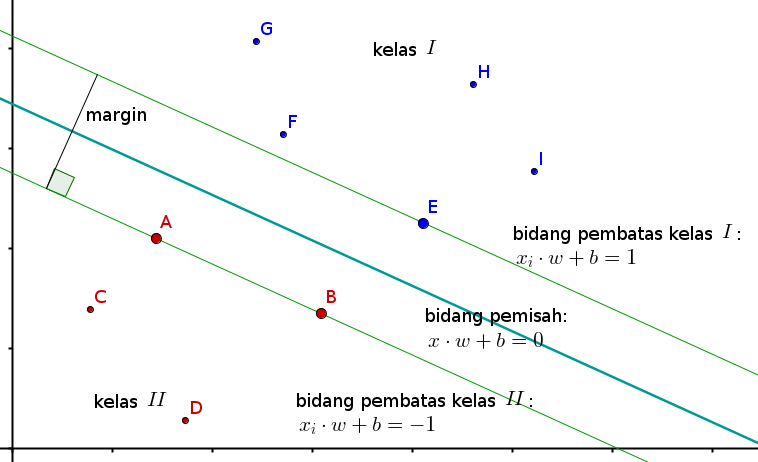
\includegraphics[width=\figurewidth]{svm}
	\caption{Ilustrasi SVM (lingkaran yang lebih besar menandakan \textit{support vector})}
	\label{gbr:studi_svm}
\end{figure}

SVM bekerja efektif pada data yang \textit{linearly separable}. Secara geometri, hal tersebut berarti terdapat sebuah garis/bidang lurus yang dapat memisahkan kedua kelas. Bidang pembatas yang ingin dicari oleh SVM diberikan oleh persamaan vektor \ref{eq:bidang_pemisah},
\begin{equation} \label{eq:bidang_pemisah}
\vec{x} \cdot \vec{w} + b = 0
\end{equation}
dengan $\vec{w}$ adalah vektor yang tegak lurus dengan bidang pembatas dan $b$ adalah jarak dari titik origin $O(0,0)$. Semua \textit{instance} yang berada di atas bidang pemisah harus memenuhi $\vec{x_i} \cdot \vec{w} + b > 0$ sementara yang berada di bawah bidang pemisah harus memenuhi $\vec{x_i} \cdot \vec{w} + b < 0$. Sederhananya, fungsi yang menentukan kelas/label dari \textit{instance} $\vec{x_i}$ diberikan oleh persamaan \ref{eq:fungsi_klasifikasi},
\begin{equation} \label{eq:fungsi_klasifikasi}
f(\vec{x_i}) = sign(\vec{x_i} \cdot \vec{w} + b)
\end{equation}
dengan $sign(\vec{x}) = -1$ jika $x < 0$ dan $sign(\vec{x}) = +1$ jika $x > 0$.

Sebuah bidang pembatas harus menjaga konsistensi dari data latih. Maksudnya adalah setiap \textit{instance} harus berada pada kelas yang sesuai dengan labelnya masing-masing. Hal tersebut dapat diperiksa menggunakan rumus \ref{eq:fungsi_pembatas},
\begin{equation} \label{eq:fungsi_pembatas}
y_i(\vec{x_i} \cdot \vec{w} + b) \geq 1
\end{equation}
dengan $y_i$ menyatakan label dari \textit{instance} $\vec{x_i}$. Selain itu, bidang pembatas juga harus memisahkan kedua kelas/label sejauh-jauhnya. Jarak antara bidang pembatas kedua kelas disebut dengan margin. Besar margin didapatkan dengan rumus \ref{eq:margin},
\begin{equation} \label{eq:margin}
m = \frac{2}{|\vec{w}|^2}
\end{equation}
dengan $|\vec{w}|$ menyatakan besar norma dari vektor $\vec{w}$.

Dengan penjelasan tersebut, permasalahan dapat dirangkum menjadi meminimalkan nilai dari $\frac{1}{2}|\vec{w}|^2$ dengan batasan $y_i(\vec{x_i} \cdot \vec{w} + b) \geq 1$. SVM menyelesaikan permasalahan tersebut dengan menentukan terlebih dahulu \textit{instance} yang akan dilewati oleh bidang pembatas dari masing-masing kelas, yaitu semua \textit{instance} yang memenuhi persamaan \ref{eq:support_vector},
\begin{equation} \label{eq:support_vector}
|\vec{x_i} \cdot \vec{w} + b| = 1.
\end{equation}
\textit{Instance} yang memenuhi persamaan tersebut disebut sebagai \textit{support vector}.

Bagaimanapun, cara tersebut hanya akan berhasil menangani data yang \textit{linearly separable}. Untuk data yang tidak \textit{linearly separable}, SVM menggunakan fungsi pemetaan yang memetakan input $\vec{x_i}$ ke dimensi yang lebih tinggi (biasa dilambangkan dengan $\phi(\vec{x_i})$). Selain itu, dapat juga ditambahkan variabel eror $\xi_i$ dan konstanta penalti $C$ untuk menangani adanya \textit{instance} dalam data latih yang berlabel salah. \textit{Instance} yang seperti itu disebut dengan \textit{noise}. Dengan demikian, permasalahan berubah menjadi meminimalkan nilai dari $\frac{1}{2}|\vec{w}|^2 + C\sum_{i} \xi_i$ dengan batasan $y_i(\phi(\vec{x_i}) \cdot \vec{w} + b) \geq 1 - \xi_i$.

Sayangnya, penggunaan fungsi pemetaan memakan biaya komputasi yang tinggi sehingga digunakanlah \textit{kernel trick}, $K(\vec{x_i}, \vec{x_j}) = \phi(\vec{x_i})\phi(\vec{x_j})$, untuk mengurangi beban komputasi. Beberapa fungsi kernel yang umum digunakan diberikan pada Tabel \ref{tbl:studi_kernel}. Dengan memformulasikan permasalah menggunakan formula Lagrange, didapatkan fungsi untuk klasifikasi sebagai persamaan \ref{eq:fungsi_klasifikasi_lagrange},
\begin{equation} \label{eq:fungsi_klasifikasi_lagrange}
f(\vec{x}) = \sum_i \alpha_i y_i K(\vec{x_i}, \vec{x}) + b
\end{equation}
dengan $\alpha$ disebut dengan $dual parameter$. \textit{Support vector} dapat diidentifikasi melalui $\alpha_i > 0$. Hipotesis yang dihasilkan oleh SVM berupa kumpulan \textit{support vector} dengan nilai $\alpha$-nya.

\begin{table}[htbp]
	\centering
	\caption{Fungsi kernel dalam SVM}
	\label{tbl:studi_kernel}
	\begin{tabular}{|p{\textwidth/4}|p{\textwidth/2}|}
		\hline
		\textbf{Fungsi Kernel} & \textbf{Formula ($K(x_i, x_j)$)}\\ \hline
		Linear & $x_i^T x_j$\\ \hline
		Polinomial & $\left( \gamma x_i^T x_j + r \right)^p, \quad \gamma > 0$\\ \hline
		RBF & $\exp\left( -\gamma \left| x_i - x_j \right|^2 \right), \quad \gamma > 0$\\ \hline
		Sigmoid & $\tanh\left( \gamma x_i^T x_j + r \right)$\\ \hline
	\end{tabular}
\end{table}

SVM sudah dicoba dalam banyak domain penelitian, seperti pengenalan tulisan tangan, klasifikasi teks, klasifikasi gambar, dan bioinformasi. \textcite{christianini} menyebutkan bahwa SVM memiliki kinerja yang menjadi \textit{state-of-the-art} dalam menyelesaikan persoalan dunia nyata. Selain itu, \textcite{vapnik} juga memaparkan 3 kelebihan SVM dipandang dari sisi pembelajaran mesin, yaitu
\begin{inparaenum}[(1)]
\item bersifat universal karena menggunakan fungsi kernel yang dapat diubah sesuai kebutuhan,
\item memiliki batas atas eror yang kecil, dan
\item memiliki kinerja yang cepat.
\end{inparaenum}

\subsection{Teknik Ekstraksi Istilah Dwibahasa}
Pembuatan kamus dwibahasa secara otomatis dapat dilakukan dengan memanfaatkan ATR. ATR digunakan untuk melakukan ekstraksi istilah-istilah yang berpotensi menjadi kata yang penting (kata kunci) dan membentuk suatu daftar istilah yang koheren (logis dan konsisten). Daftar istilah tersebut nantinya akan menjadi entri kamus dwibahasa. Terdapat 2 jenis teknik yang dapat dipakai untuk melakukan ATR, yaitu \parencite{ananiadou}
\begin{inparaenum}[(1)]
\item teknik linguistik dan
\item teknik nonlinguistik (statistik/probabilitas).
\end{inparaenum}

Saat ini, sudah banyak penelitian yang terkait dengan ekstraksi istilah dari korpus dengan berbagai macam teknik. Pada kenyataannya, kebanyakan teknik yang digunakan telah menggabungkan teknik linguistik dan nonlinguistik. Beberapa teknik/pendekatan yang berpotensi untuk diadopsi untuk bahasa Indonesia dipaparkan berikut ini.

\subsubsection{Pendekatan Linguistik}
\label{subsubbab:studi_linguistik}
Pendekatan linguistik memanfaatkan karakteristik bahasa, seperti Pos \textit{tag}, pola, dan aturan bahasa (\textit{grammar}). Salah satu penelitian mengenai ATR yang murni memakai pendekatan linguistik dilakukan oleh \textcite{ananiadou}. Tujuan penelitian tersebut adalah untuk mengekstrak istilah-istilah dalam domain farmasi. Idenya adalah dengan membentuk sebuah aturan pembentukan istilah/kata dalam level morfologi berupa awalan, akar kata, dan akhiran. Selain itu, \textcite{ananiadou} juga mempertimbangkan banyaknya pemakaian awalan/kata/akhiran serapan dari bahasa Latin dan Yunani (\textit{neoclassical element}) dalam pembuatan aturan.

Di samping itu, \textcite{tsuji} memanfaatkan transliterasi untuk melakukan ekstraksi pasangan kata bahasa Jepang-Prancis. Idenya adalah dengan memanfaatkan kata bahasa Inggris yang diserap oleh kedua bahasa. Kata serapan biasanya memiliki ciri-ciri morfologi (huruf, bunyi huruf, dll) yang mirip dengan kata dari bahasa akarnya. Penelitian tersebut mengikuti penelitian sebelumnya yang menggunakan teknik yang sama namun ditujukan untuk pasangan kata bahasa Inggris-Jepang. Teknik tersebut menghasilkan tingkat presisi 80\% untuk pasangan kata bahasa Jepang-Prancis. Teknik tersebut menjanjikan untuk diadopsi untuk bahasa Indonesia karena bahasa Indonesia juga menyerap banyak istilah dari bahasa asing (terutana Inggris), terutama dalam bidang pendidikan, pemerintahan, dan industri.

Bagaimanapun, terdapat batasan dalam pendekatan tersebut bahwa bahasa asal dan bahasa sasaran harus memiliki banyak kata yang seakar. Dengan kata lain, kinerja dari pendekatan ini bergantung pada karakteristik morfologi istilah dari masing-masing bahasa. Penelitian yang dilakukan oleh \textcite{fujii} memberikan hasil \textit{trade-off} terhadap nilai presisi dan nilai \textit{recall}. Sebagai contoh, presisi 50.0\% memiliki \textit{recall} 8.5\% sedangkan \textit{recall} 69.5\% memiliki presisi hanya 1.2\%. Hal tersebut dapat ditangani menggunakan sebuah kamus dwibahasa tambahan.

Secara umum, teknik tersebut dapat dibagi menjadi 2 buah proses utama, yaitu
\begin{inparaenum}[(1)]
\item pembangunan aturan transliterasi dan
\item ekstraksi pasangan kata transliterasi.
\end{inparaenum}
Berikut ini dipaparkan langkah-langkah detail untuk setiap proses. Istilah "kata katakana" digunakan untuk menyatakan kata dalam bahasa Jepang yang ditulis dalam huruf katakana (yang biasanya dipakai untuk menuliskan kata serapan).

\paragraph{Pembangunan Aturan Transliterasi} ~\\
Salah satu hal krusial dalam teknik tersebut adalah harus tersedianya aturan transliterasi dari bahasa Jepang ke bahasa Prancis. Pembangunan aturan transliterasi dilakukan dengan cara
\begin{enumerate}
\item uraikan kata katakana dari sebuah daftar ke dalam kumpulan \textit{mora unit},
\item berdasarkan pasangan kata bahasa Prancisnya, buat aturan transliterasi untuk setiap \textit{mora unit} secara manual, dan
\item ulangi langkah 1-2 untuk semua pasangan kata dalam daftar dan urutkan transliterasi berdasarkan frekuensi kemunculannya (yang paling sering yang paling pertama).
\end{enumerate}

Daftar yang digunakan untuk pembangunan aturan transliterasi tidak hanya dari pasangan bahasa Jepang-Prancis, tetapi juga dari pasangan bahasa Inggris-Jepang. Daftar pasangan istilah bahasa Jepang-Prancis didapatkan dari \textit{Concorde Japanese-French Dictionary} sedangkan pasangan istilah bahasa Inggris-Jepang didapatkan dari EDICT\footnote{\url{http://www.edrdg.org/jmdict/edict.html}}. \textcite{tsuji} menjelaskan bahwa penggunaan bahasa Inggris disebabkan pasangan istilah bahasa Inggris-Jepang lebih mudah ditemukan dan karakteristiknya tidak berbeda jauh dengan karakteristik bahasa Prancis.

\paragraph{Ekstraksi Pasangan Kata Transliterasi} ~\\
Setelah didapatkan aturan transliterasi, korpora dwibahasa (Jepang-Prancis) digunakan untuk menentukan padanan kata bahasa Prancis diketahui sebuah kata dalam bahasa Jepang. Pencarian kata bahasa Prancis dihitung menggunakan ukuran $Dice$ (yang melibatkan panjang karakter yang mirip) alih-alih komparasi karakter demi karakter. Hal tersebut disebabkan kata bahasa Prancis dalam korpus mungkin tidak muncul sebagai kandidat yang dibangkitkan dari aturan transliterasi. Langkah-langkahnya adalah sebagai berikut.
\begin{enumerate}
\item Ambil sebuah kata katakana, misalnya $J$, dan uraikan ke dalam kumpulan \textit{mora unit};
\item Dengan aturan transliterasi yang telah dibangun, bangkitkan semua kandidat transliterasi yang mungkin. Misalkan $T_i(J)$ menyatakan kandidat transliterasi ke-$i$;
\item Ambil kata bahasa Prancis, misalkan $F$, yang muncul bersamaan dengan $J$ dalam korpus. Cari nilai $LCS$-nya dengan setiap $T_i(J)$ (misalkan dilambangkan dengan $LCS(F,T_i(J))$). $LCS$ merupakan singkatan dari \textit{Longest Common Subsequence} dan mengembalikan barisan karakter terpanjang yang muncul terurut (bukan berurutan) dalam kedua kata. Misalkan kedua kata tersebut adalah $X = x_1x_2 \ldots x_m$ dan $Y = y_1y_2 \ldots y_n$ dengan $x_i,y_i$ melambangkan sebuah karakter. Misalkan juga $X_i = x_1x_2 \ldots x_i$ dan $Y_j = y_1y_2 \ldots y_j$. $LCS$ (atau dapat disingkat dengan $L$) dapat dicari dengan rumus rekursi pada persamaan \ref{eq:lcs}.
\begin{equation} \label{eq:lcs}
	L(X_i,Y_j) = \left\{
		\begin{array}{l l}
			\emptyset &\quad \text{jika $i = 0$ atau $j = 0$}\\
			L(X_{i-1},Y_{j-1}) \cup x_i &\quad \text{jika $x_i = y_j$}\\
			lg \left( L(X_{i-1},Y_j), L(X_i,Y_{j-1}) \right) &\quad \text{jika $x_i \neq y_j$}
		\end{array}
	\right.
\end{equation}
dengan fungsi $lg$ mengembalikan barisan terpanjang;
\item Hitung nilai dari peluang $p$ dengan persamaan \ref{eq:p}:
\begin{equation} \label{eq:p}
	P(J,F) = \max_i \left( Dice \left( len \left( LCS(T_i(J), F) \right), len \left( T_i(J) \right), len \left( F \right) \right) \right)
\end{equation}
dan ambil $J$ dan $F$ sebagai pasangan translasi jika nilainya melebihi \textit{threshold}. Fungsi $len$ menyatakan panjang karakter dari kata dan rumus $Dice$ diberikan oleh persamaan \ref{eq:dice}.
\begin{equation} \label{eq:dice}
	Dice(k,m,n) = k \times \frac{2}{m + n}.
\end{equation}
\end{enumerate}

\begin{table}[htbp]
	\centering
	\caption{Contoh aturan transliterasi}
	\label{tbl:studi_transliterasi}
	\begin{tabular}{|c|c|c|}
		\hline
		\begin{CJK}{UTF8}{min} グ \end{CJK} & \begin{CJK}{UTF8}{min} ラ \end{CJK} & \begin{CJK}{UTF8}{min} フ \end{CJK}\\ \hline
		g & ra & f\\
		gue & la & phe\\
		gu & l & ff\\
		& lu & fe\\
		& r & \\
		& ler & \\ \hline
	\end{tabular}
\end{table}

Sebagai ilustrasi \parencite{tsuji}, misalkan aturan transliterasi diberikan oleh Tabel \ref{tbl:studi_transliterasi} dan bahasa Jepang yang diekstrak adalah $J:$\begin{CJK}{UTF8}{min}グラフ\end{CJK}. Langkah-langkah selanjutnya adalah sebagai berikut.
\begin{enumerate}
\item $J:$\begin{CJK}{UTF8}{min}グラフ\end{CJK} $\implies$ \begin{CJK}{UTF8}{min}グ,ラ,フ\end{CJK}.
\item Banyaknya kandidat transliterasi yang dibangkitkan ada $3 \times 6 \times 4 = 72$ buah meliputi $graf, graphe, graff, grafe, \ldots, gulerff, gulerfe$.
\item Misalkan kata bahasa Prancis $F:graphe$ muncul bersamaan dengan kata katakana tersebut.
\item Hitung nilai dari fungsi $P$ dan ambil kandidat dengan nilai $Dice$ tertinggi.
\[
	\begin{aligned}
		P(&\text{\begin{CJK}{UTF8}{min}グラフ\end{CJK}},graphe)\\
		&= \max(Dice(len(LCS(graf, graphe)), len(graf), len(graphe)),\\
		&\quad Dice(len(LCS(graphe, graphe)), len(graphe), len(graphe)),\\
		&\quad Dice(len(LCS(graff, graphe)), len(graff), len(graphe)),\\
		&\quad \vdots\\
		&\quad Dice(len(LCS(gulerfe, graphe)), len(gulerfe), len(graphe)))\\
		&= \max(0.60, 1.00, 0.55, \ldots, 0.31)\\
		&= 1.00
	\end{aligned}
\]
sehingga \begin{CJK}{UTF8}{min}グラフ\end{CJK} dan $graphe$ kemungkinan besar merupakan sebuah pasangan istilah yang ekivalen.
\end{enumerate}

\subsubsection{Pendekatan Statistik}
\label{subsubbab:studi_statistik}
Pendekatan statistik menggunakan informasi \textit{$n$-gram} dan perhitungan statistik seperti tingkat persebaran kata dalam dokumen. Salah satu contohnya adalah penelitian yang dilakukan oleh \textcite{rapp}. Idenya adalah jika kata $A$ dan $B$ muncul bersama lebih sering dari yang diharapkan dalam bahasa asal, translasi keduanya dalam bahasa sasaran juga akan muncul bersama-sama lebih sering dari yang diharapkan.

Teknik tersebut mengasumsikan bahwa terdapat korelasi kemunculan kata dalam teks yang berbeda bahasa. \textcite{rapp} merepresentasikan frekuensi kemunculan bersama sebagai sebuah matriks berukuran $n \times n$ (\textit{$n$-gram}). Dua buah matriks akan menjadi pasangan translasi satu dengan yang lain jika kedua matriks tersebut memiliki jarak \textit{city-block} yang terdekat.

Berbeda dengan \textcite{rapp}, \textcite{yu} justru menggunakan ukuran \textit{context heterogeneity similarity} yang diadopsi dari penelitian yang dilakukan oleh \textcite{fung}. \textcite{fung} mengajukan bahwa \textit{context heterogeneity similarity} adalah fitur/ciri-ciri yang lebih menonjol (\textit{salient}) dibandingkan frekuensi kemunculan bersama.

Konsepnya adalah sebuah kata/istilah dalam sebuah domain hanya memiliki kata-kata tertentu yang dapat langsung mendahului atau mengikutinya. Semakin umum sebuah kata/istilah (bukan istilah penting dalam domain), semakin banyak kata yang dapat langsung mendahului atau mengikutinya. Dengan demikian, nilai \textit{context heterogeneity similarity} dari kata tersebut semakin besar. Sebaliknya, istilah dalam domain hanya memiliki sedikit kata yang dapat langsung mendahului atau mengikutinya sehingga nilai \textit{context heterogeneity similarity} dari kata tersebut kecil. \textit{Context heterogeneity similarity} dari sebuah kata $W$ dinyatakan sebagai sebuah vektor 2 dimensi $\vec{h}$ sebagaimana yang ditunjukkan pada persamaan \ref{eq:context_heterogeneity}:
\begin{equation} \label{eq:context_heterogeneity}
\vec{h} = (h_{kiri}, h_{kanan})
\end{equation}
dengan
\[
\begin{aligned}
	h_{kiri}(W) &= \frac{\text{banyak kata berbeda yang langsung mendahului $W$}}{\text{banyak kemunculan $W$}} \quad \text{dan}\\
	h_{kanan}(W) &= \frac{\text{banyak kata berbeda yang langsung mengikuti $W$}}{\text{banyak kemunculan $W$}}.
\end{aligned}
\]

\textcite{yu} kemudian menyempurnakan fitur tersebut dengan menambah fitur \textit{dependency heterogeneity similarity}. Fitur tersebut diajukan untuk menangani masalah terdapat kata yang muncul dalam konteks yang serupa, namun bukan pasangan translasi. \textit{Dependency heterogeneity similarity} dari sebuah kata $W$ dinyatakan sebagai sebuah vektor 4 dimensi $\vec{d}$ sebagaimana yang ditunjukkan pada persamaan \ref{eq:dependency_heterogeneity}:
\begin{equation} \label{eq:dependency_heterogeneity}
\vec{d} = (d_{NMODHead}, d_{SUBHead}, d_{OBJHead}, d_{NMODMod})
\end{equation}
dengan
\[
\begin{aligned}
	d_{NMODHead} &= \frac{\text{banyak \textit{head} berbeda dari $W$ dengan label NMOD}}{\text{banyak \textit{head} dari $W$ dengan label NMOD}},\\
	d_{SUBHead} &= \frac{\text{banyak \textit{head} berbeda dari $W$ dengan label SUB}}{\text{banyak \textit{head} dari $W$ dengan label SUB}},\\
	d_{OBJHead} &= \frac{\text{banyak \textit{head} berbeda dari $W$ dengan label OBJ}}{\text{banyak \textit{head} dari $W$ dengan label OBJ}}, \text{ dan}\\
	d_{NMODmod} &= \frac{\text{banyak \textit{modifier} berbeda dari $W$ dengan label NMOD}}{\text{banyak \textit{modifier} dari $W$ dengan label NMOD}}.
\end{aligned}
\]

Penentuan pasangan translasi dilakukan dengan menghitung nilai \textit{context heterogeneity similarity} dan \textit{dependency heterogeneity similarity} untuk setiap kandidat istilah dari masing-masing bahasa. Penentuan pasangan translasi atau bukan dilakukan dengan mengukur jarak \textit{euclidean}. Pasangan istilah yang diambil sebagai pasangan translasi adalah pasangan istilah dengan jarak \textit{euclidean} terkecil.

\textcite{aker} menggunakan pendekatan yang berbeda dari yang lain, yaitu dengan memandang ATR sebagai permasalahan klasifikasi. Hasil yang didapatkan adalah hingga 83\% pasangan istilah yang dibangkitkan merupakan translasi yang tepat. Pendekatan ini mengasumsikan bahwa terdapat cara untuk mengekstrak \textit{monolingual term} baik untuk bahasa asal maupun untuk bahasa sasaran. Dibandingkan pendekatan linguistik yang dibahas pada Subbab \ref{subsubbab:studi_linguistik}, teknik yang dipakai dalam pendekatan ini lebih sederhana. Ringkasnya, cara yang digunakan adalah
\begin{enumerate}
\item memasangkan setiap istilah yang diekstrak dari korpus bahasa asal dengan setiap istilah yang diekstrak dari korpus bahasa sasaran,
\item mengekstrak fitur dari setiap pasangan istilah, dan
\item berdasarkan fitur yang diekstrak, melakukan klasifikasi apakah pasangan istilah tersebut ekuivalen atau tidak (\textit{binary classification}).
\end{enumerate}

Fitur yang dipakai dapat dibagi menjadi 3 kategori, yaitu
\begin{inparaenum}[(1)]
\item fitur berbasis kamus,
\item fitur berbasis kognat, dan
\item gabungan keduanya.
\end{inparaenum}
Untuk mengekstrak fitur berbasis kamus, dibutuhkan sebuah kamus dwibahasa. Fitur berbasis kamus memiliki arah, yaitu bergantung pada pemilihan mana yang menjadi bahasa asal dan mana yang menjadi bahasa sasaran. Oleh karena itu, total fitur berbasis kamus ada $2 \times 6 + 1 = 13$ buah dengan satu fitur adalah rata-rata dari 2 kemungkinan pemilihan pasangan bahasa asal-sasaran sebagaimana yang dijelaskan berikut ini.
\begin{enumerate}
\item \textit{isFirstWordTranslated}: fitur \textit{boolean} yang menandakan apakah kata pertama dari istilah bahasa asal merupakan translasi kata pertama dari istilah bahasa sasaran. Contohnya, pasangan istilah (automatic term recognition, pengenalan istilah otomatis) bernilai $false$ sedangkan pasangan istilah (rule of thumb, aturan ibu jari) bernilai $true$.
\item \textit{isLastWordTranslated}: fitur \textit{boolean} yang menandakan apakah kata terakhir dari istilah bahasa asal merupakan translasi kata terakhir dari istilah bahasa sasaran. Contohnya, pasangan istilah (automatic term recognition, pengenalan istilah otomatis) bernilai $false$ sedangkan pasangan istilah (rule of thumb, aturan ibu jari) bernilai $true$.
\item \textit{percentageOfTranslatedWords}: persentasi banyak kata dari istilah bahasa asal yang memiliki translasi dalam istilah bahasa sasaran. Contohnya, pasangan istilah (automatic term recognition, pengenalan istilah) bernilai $\frac{2}{3} \times 100\% = 66,57\%$.
\item \textit{percentageOfNotTranslatedWords}: persentasi banyak kata dari istilah bahasa asal yang tidak memiliki translasi dalam istilah bahasa sasaran. Contohnya, pasangan istilah (automatic term recognition, pengenalan istilah) bernilai $\frac{1}{3} \times 100\% = 33,33\%$.
\item \textit{longestTranslatedUnitInPercentage}: rasio (dalam persen) banyak kata berurutan yang terpanjang dari istilah bahasa asal yang memiliki translasi dalam istilah bahasa sasaran terhadap banyak kata seluruhnya dari istilah bahasa asal. Contohnya, pasangan istilah (responsive web user interface development, pengembangan antarmuka yang responsif) bernilai $\frac{2}{5} \times 100\% = 40\%$.
\item \textit{longestNotTranslatedUnitInPercentage}: rasio (dalam persen) banyak kata berurutan yang terpanjang dari istilah bahasa asal yang tidak memiliki translasi dalam istilah bahasa sasaran terhadap banyak kata seluruhnya dari istilah bahasa asal. Contohnya, pasangan istilah (responsive web user interface development, antarmuka yang responsif) bernilai $\frac{2}{5} \times 100\% = 40\%$.
\item \textit{averagePercentageOfTranslatedWords}, yaitu rata-rata dari \textit{percentageOfTranslatedWords} untuk 2 kemungkinan pemilihan pasangan bahasa asal-sasaran. Contohnya, Contohnya, pasangan istilah (responsive web user interface development, pengembangan antarmuka yang responsif) memiliki nilai \textit{percentageOfTranslatedWords} $\frac{2}{5} \times 100\% = 40\%$ sementara pasangan istilah (pengembangan antarmuka yang responsif, responsive web user interface development) memiliki nilai $\frac{2}{4} \times 100\% = 50\%$. Jadi, nilai dari \textit{averagePercentageOfTranslatedWords} adalah $(40\% + 50\%) / 2 = 45\%$.
\end{enumerate}

Fitur berbasis kognat digunakan untuk menangani istilah yang tidak dapat ditangani oleh kamus, seperti \textit{named entity} dan istilah khusus. \textcite{aker} menyebutkan, "Metode kognat mengasumsikan bahwa bahasa asal dan bahasa sasaran yang dibandingkan menggunakan jenis karakter yang sama". Oleh karena itu, dibuat sebuah pemetaan karakter dari bahasa asal ke bahasa sasaran dan sebaliknya jika kedua bahasa menggunakan karakter yang berbeda. Terdapat 5 buah fitur kognat, sehingga totalnya terdapat $5 + 2 \times 5 = 15$ berupa 5 fitur tanpa pemetaan karakter, 5 fitur dengan karakter bahasa asal, dan 5 fitur dengan karakter bahasa sasaran. Berikut ini adalah detail fitur berbasis kognat yang digunakan.
\begin{enumerate}
\item \textit{Longest Common Subsequence Ratio} (LCSR):
\begin{equation}
	LCSR(X,Y) = \frac{len(LCS(X,Y))}{\max(len(X), len(Y))}
\end{equation}
dengan $LCS(X,Y)$ mengembalikan barisan karakter terpanjang yang muncul terurut (bukan berurutan) dalam kedua kata. Contohnya, \[ LCS(efisien,efficient) = efiien \] maka
\[
	\begin{aligned}
		LCSR(efisien,efficient) &= \frac{len(efiien)}{\max(len(efisien), len(efficient))}\\
		&= \frac{6}{\max(7,9)}\\
		&= \frac{6}{9}\\
		&= 0,67.
	\end{aligned}
\]
\item \textit{Longest Common Substring Ratio} (LCSTR):
\begin{equation}
	LCSTR(X,Y) = \frac{len(LCST(X,Y))}{\max(len(X), len(Y))}
\end{equation}
dengan $LCST(X,Y)$ menyatakan \textit{substring} (barisan karakter berurutan) terpanjang yang ada baik dalam $X$ maupun $Y$. Contohnya, \[ LCST(efisien,efficient) = ien \] maka
\[
	\begin{aligned}
		LCSTR(efisien,efficient) &= \frac{len(ien)}{\max(len(efisien), len(efficient))}\\
		&= \frac{3}{\max(7,9)}\\
		&= \frac{3}{9}\\
		&= 0,33.
	\end{aligned}
\]
\item \textit{Dice Similarity}:
\begin{equation}
	dice = 2 \times \frac{len(LCST(X,Y))}{len(X) + len(Y)}.
\end{equation}
\item \textit{Needleman Wunsch Distance} (NWD):
\begin{equation}
	NWD = \frac{len(LCST(X,Y))}{\min(len(X), len(Y))}.
\end{equation}
\item \textit{Levenshtein Distance} (LD):
\begin{equation}
	LD_{normalized}(X,Y) = 1 - \frac{LD(X,Y)}{\max(len(X), len(Y))}.
\end{equation}
Sebenarnya, \textit{levenshtein distance} menyatakan banyak operasi-satu-karakter minimum yang harus dilakukan untuk mengubah satu \text{string} menjadi \textit{string} yang lain. Operasi yang terdefinisi antara lain \textit{insertion} (menambah 1 karakter), \textit{deletion} (menghapus 1 karakter), dan \textit{substitution} (mengubah 1 karakter). Untuk penyeragaman dengan fitur kognat yang lain, \textcite{aker} menormalkannya menjadi bentuk tersebut. Contohnya, \[ LD(efisien,efficient) = 3 \] meliputi 2 operasi \textit{insertion} (huruf 'f' dan 't') dan 1 operasi \textit{substitution} (huruf 's' menjadi huruf 'c'). Jadi,
\[
	\begin{aligned}
		LD_{normalized}(efisien,efficient) &= 1 - \frac{LD(efisien,efficient)}{\max(len(efisien), len(efficient))}\\
		&= 1 - \frac{3}{\max(7,9)}\\
		&= 0,67.
	\end{aligned}
\]
\end{enumerate}

Fitur berbasis gabungan kamus dan kognat juga dipertimbangkan dalam pembelajaran. Untuk mengekstrak fitur tersebut, didefinisikan bahwa sebuah kata dari bahasa asal memiliki translasi dalam bahasa sasaran jika terdapat pasangan kata tersebut di dalam kamus. Didefinisikan juga bahwa sebuah kata dari bahasa asal memiliki transliterasi dalam bahasa sasaran jika salah satu fitur kognatnya bernilai lebih dari $0,7$. Fitur gabungan juga memiliki arah, sehingga totalnya ada $2 \times 5 = 10$ fitur gabungan. Berikut ini adalah daftar fitur gabungan yang dipakai.
\begin{enumerate}
\item \textit{isFirstWordCovered}: fitur bernilai \textit{boolean} yang menandakan apakah kata pertama dari istilah bahasa asal memiliki translasi atau transliterasi dalam istilah bahasa sasaran.
\item \textit{isLastWordCovered}: fitur bernilai \textit{boolean} yang menandakan apakah kata terakhir dari istilah bahasa asal memiliki translasi atau transliterasi dalam istilah bahasa sasaran.
\item \textit{percentageOfCoverage}: persentasi dari banyak kata dari istilah bahasa asal yang memiliki translasi atau transliterasi dalam istilah bahasa sasaran.
\item \textit{percentageOfNonCoverage}: persentasi dari banyak kata dari istilah bahasa asal yang tidak memiliki translasi atau transliterasi dalam istilah bahasa sasaran.
\item \textit{difBetweenCoverageAndNonCoverage}: selisih dari 2 fitur terakhir (\textit{percentageOfCoverage} dan \textit{percentageOfNonCoverage}).
\end{enumerate}

\subsection{Penelitian Terkait}
\label{studi_terkait}
Pembangunan kamus dwibahasa Indonesia-Jepang pernah dilakukan sebelumnya oleh \textcite{limanthie}. Teknik yang digunakannya cukup intuitif, yaitu dengan melihat seberapa sering sepasang istilah bahasa Indonesia-Jepang muncul bersamaan di dalam korpus. Pasangan istilah dengan frekuensi kemunculan bersama yang tinggi tentunya cenderung merupakan pasangan translasi. Terdapat 6 variabel yang diperhatikan dalam eksperimen yang dilakukannya, yaitu
\begin{inparaenum}[(1)]
\item ada-tidaknya \gls{stopword},
\item lingkup korpus: per dokumen atau seluruh dokomen,
\item jarak antarkata,
\item jenis kata: tidak dibatasi atau kata benda saja,
\item metode perhitungan frekuensi yang dipakai: \textit{single co-occurrence} atau \textit{multi co-occurrence}, dan
\item menambahkan judul artikel ke dalam kamus awal atau tidak.
\end{inparaenum}

Eksperimen dilakukan dengan korpora \textit{comparable} yang dikumpulkan dari Wikipedia dengan domain \textit{computer science}. Terdapat 152 pasangan artikel bahasa Indonesia-Jepang yang digunakan dalam pengujian \parencite{limanthie}. Pemrosesan seluruh dokumen memiliki sisi positif dapat lebih banyak pasangan istilah yang terekstrak, namun konteks dari 152 artikel tersebut tercampur. Di lain pihak, pemrosesan per dokumen memiliki konteks yang fokus sehingga dapat memberikan hasil yang lebih tepat, namun pasangan istilah yang terekstrak kurang beragam.

Selain itu, \textcite{limanthie} juga menggunakan kamus awal untuk membantu mencari kandidat pasangan istilah. Entri kamus berupa kata-kata umum dan dipakai sebagai acuan (\textit{anchor}) untuk membangkitkan kandidat pasangan istilah. Contohnya, diketahui dari kamus awal bahwa kata "bahasa" memiliki padanan kata "\begin{CJK}{UTF8}{min}言語\end{CJK}" dalam bahasa Jepang. Dari korpus, didapatkan kata "pemrograman" sering muncul berdekatan dengan kata "bahasa" sedangkan kata "\begin{CJK}{UTF8}{min}プログラミング\end{CJK}" sering muncul berdekatan dengan kata "\begin{CJK}{UTF8}{min}言語\end{CJK}". Secara intuitif, dapat disimpulkan bahwa pasangan kata (pemrograman,\begin{CJK}{UTF8}{min}プログラミング\end{CJK}) mungkin sebuah pasangan translasi dan dapat diambil sebagai sebuah kandidat. Kamus awal tentunya masih memiliki sedikit entri dan dapat diperbanyak dengan menambahkan judul artikel ke dalam kamus. Hal tersebut mungkin berhasil karena judul artikel Wikipedia biasanya adalah translasi langsung satu dengan yang lain.

Terdapat 2 pendekatan yang dilakukan \textcite{limanthie} untuk menghitung frekuensi kemunculan, yaitu
\begin{inparaenum}[(1)]
\item \textit{single co-occurrence} dan
\item \textit{multi co-occurrence}.
\end{inparaenum}
\textit{Single co-occurrence} hanya menggunakan satu kata acuan sedangkan \textit{multi co-occurrence} menggunakan 2 atau lebih kata acuan. \textcite{limanthie} kemudian membuat 7 buah eksperimen yang ditujukan untuk mencari kondisi yang paling kondusif untuk melakukan ekstraksi istilah. Ketujuh kondisi tersebut beserta hasilnya diberikan pada Tabel \ref{tbl:studi_eksperimen_limanthie}.

\begin{table}[htbp]
	\centering
	\caption{Hasil eksperimen yang dilakukan \textcite{limanthie}}
	\label{tbl:studi_eksperimen_limanthie}
	\begin{tabular}{|r|p{\tablewidth/2}|p{\tablewidth/3}|}
		\hline
		\textbf{No.} & \textbf{Perubahan} & \textbf{Hasil}\\ \hline
		\tableitem & Akurasi awal. & Tidak ada.\\ \hline
		\tableitem & Menghilangkan \textit{stop word}. & Lebih baik \textit{stop word} dihilangkan.\\ \hline
		\tableitem & Mengubah pembentukan daftar pasangan kata menjadi per dokumen. & Lebih baik lingkup korpus per dokumen.\\ \hline
		\tableitem & Memproses kata benda saja. & Lebih baik hanya kata benda yang diproses untuk jarak 3 kata.\\ \hline
		\tableitem & Mempertimbangkan \textit{multi co-occurrence}. & Lebih baik \textit{single co-occurrence}.\\ \hline
		\tableitem & Menambah judul artikel pada kamus awal. & Tidak ada perbedaan.\\ \hline
		\tableitem & Melakukan iterasi. & Lebih baik dengan iterasi.\\ \hline
	\end{tabular}
\end{table}

Selain teknik tersebut, pembuatan kamus dwibahasa juga dapat dilakukan dengan bantuan pembelajaran mesin. Pendekatan tersebut dilakukan oleh \textcite{aker}. Idenya adalah dengan memandang translasi sebagai masalah klasifikasi: apakah sebuah pasangan istilah ekuivalen atau tidak. Detail mengenai teknik yang digunakan \textcite{aker} telah dijelaskan pada Subbab \ref{subsubbab:studi_statistik}. Klasifikasi dilakukan menggunakan SVM \textit{binary classifier} dengan data latih diambil dari EUROVOC\footnote{\url{http://eurovoc.europa.eu/drupal/?q=download/list_pt&cl=en}}. EUROVOC merupakan sebuah ensiklopedi (\textit{thesaurus}) multibahasa dan multidisiplin yang mencakup aktivitas dari \textit{European Union}, terutama \textit{European Parliament}. EUROVOC kini melingkupi 23 bahasa berbeda negara-negara di benua Eropa.

\textcite{aker} juga menggunakan sebuah kamus untuk mengekstrak fitur berbasis kamus. Pembuatan kamus dilakukan dengan GIZA++\footnote{\url{https://code.google.com/p/giza-pp/}}. Kamus yang dihasilkan merupakan kumpulan entri dengan format $<s, t_i, p_i>$ dengan $s$ menyatakan kata dari bahasa asal, $t_i$ adalah translasi ke-$i$ dari $s$ dalam bahasa sasaran, dan $p_i$ adalah peluang $s$ ditranslasikan dengan $t_i$. Kemudian, kamus disaring dengan menghapus entri yang memiliki nilai peluang $p_i < 0.05$ dan entri yang mengandung \textit{stop word}. Contoh keluaran dari GIZA++ diberikan pada Tabel \ref{tbl:contoh_entri_kamus}.

\begin{table}[htbp]
	\centering
	\caption{Contoh entri kamus latih}
	\label{tbl:contoh_entri_kamus}
	\begin{tabular}{|l|l|l|}
		\hline
		\textbf{Bahasa Indonesia} & \textbf{Bahasa Jepang} & \textbf{Peluang}\\ \hline
		bahasa & \begin{CJK}{UTF8}{min}言語\end{CJK} & 0,68\\ \hline
		bahasa & \begin{CJK}{UTF8}{min}語\end{CJK} & 0,45\\ \hline
		kendaraan & \begin{CJK}{UTF8}{min}車\end{CJK} & 0,66\\ \hline
		komputer & \begin{CJK}{UTF8}{min}コンピュータ\end{CJK} & 0,99\\ \hline
		mobil & \begin{CJK}{UTF8}{min}車\end{CJK} & 0,50\\ \hline
	\end{tabular}
\end{table}

Pendekatan yang dilakukan \textcite{aker} tidak bergantung pada jenis korpora yang dipakai. Selain itu, jenis kata yang diproses tidak hanya kata benda, tetapi juga bisa kata kerja atau kata sifat. Meskipun demikian, pendekatan tersebut memerlukan \textit{monolingual term extractor} untuk masing-masing bahasa. Oleh karena itu, kinerjanya sangat bergantung pada kualitas daftar istilah yang berhasil diekstrak dari masing-masing bahasa.

Hasil akhir dari penelitian yang dilakukan \textcite{limanthie} masih memiliki akurasi kurang dari 5\% dengan banyaknya pasangan istilah translasi yang benar yang berhasil diekstrak mencapai 80 pasangan dari semua eksperimen. \textcite{limanthie} menyebutkan hal tersebut disebabkan korelasi antarartikel dalam Wikipedia yang berbeda versi bahasa sangat kecil karena beda artikel ditulis oleh beda orang. Penyebab lainnya adalah karena banyak kata memiliki kandidat translasi yang lebih dari satu, padahal kebanyakan hanya satu yang benar. Hal tersebut tentunya mengurangi akurasi kamus yang dibangun. Di lain pihak, penelitian yang dilakukan \textcite{aker} mendapatkan hasil yang bagus. Sebanyak 80\% dari pasangan istilah yang berhasil diekstrak merupakan pasangan translasi yang ekivalen.

\end{document}